% ==================================================
% 3. OddSHAP
% ==================================================
\chapter{OddSHAP}
\label{sec:oddshap}

\section{Summary}
\label{sec:oddshap:summary}

% Written by Sara; adapted from oddshap_summary.md, converted to LaTeX.

\paragraph{The core idea.}
Every set function $f: 2^{[d]} \to \mathbb{R}$ splits into an odd and an even part,
$f = f_{\mathrm{odd}} + f_{\mathrm{even}}$, where
$f_{\mathrm{odd}}(S) = \tfrac{1}{2}\left(f(S) - f(S^{c})\right)$ and
$f_{\mathrm{even}}(S) = \tfrac{1}{2}\left(f(S) + f(S^{c})\right)$. The paper's key observation
(Observation~3.1) is that the Shapley value depends only on $f_{\mathrm{odd}}$:
$\phi_i(f) = \phi_i(f_{\mathrm{odd}})$ for every player $i$. The marginal contributions of
complementary coalitions cancel the even part out when summed over all subsets.

This explains why paired sampling --- evaluating $S$ and $S^{c}$ together --- helps as much as
it does in practice. The authors show (Theorem~3.2) that under paired samples a regression
objective over a function class closed under the odd/even decomposition splits into two
independent problems, one per part. Since only the odd part matters for $\phi_i$, paired
sampling implicitly filters out irrelevant even structure. It also motivates the estimator
itself: if only $f_{\mathrm{odd}}$ has to be recovered, no budget should be spent fitting
even-order terms at all.

\paragraph{Why the Fourier basis.}
The usual regression estimators (KernelSHAP, \leverageshap{}, \polyshap{}) work in the
unanimity/Möbius basis, whose basis functions mix odd and even components. The Fourier (Walsh)
basis $\chi_T(S) = (-1)^{|S \cap T|}$ does not: $\chi_T$ is an odd function exactly when $|T|$
is odd. The authors therefore restrict a Fourier regression to odd-cardinality terms, and show
(Theorem~3.5) that the constrained regression is still consistent --- it recovers the Shapley
values through the same projection KernelSHAP and \polyshap{} use.

\paragraph{The estimator.}
Algorithm~1 has three steps.
\begin{enumerate}
    \item \textbf{Paired sampling.} Coalitions are drawn without replacement, uniformly over
        coalition sizes, and every sampled $S$ is paired with its complement $S^{c}$.
    \item \textbf{Interaction screening.} A gradient-boosted tree is fit to the sampled
        coalitions and converted to its Fourier spectrum; the odd-cardinality terms with the
        largest coefficients are kept as candidates. The candidate budget is
        $\lceil m/\eta \rceil$, where $\eta$ trades support size against regression budget.
        The paper's default is $\eta = 10$.
    \item \textbf{Sparse odd regression.} A weighted least-squares problem is solved over the
        singletons plus the selected higher-order odd terms, with the empty and full coalition
        values as exact boundary constraints --- efficiency is enforced, not approximated by
        large weights. The Shapley values follow in closed form as
        $\phi_i = -2 \sum_{T \ni i,\, |T| \text{ odd}} \beta_T / |T|$.
\end{enumerate}
If the budget cannot cover even the linear terms ($m < d\eta$), the paper falls back to reading
the Shapley values off the fitted tree with TreeSHAP.

\paragraph{What the paper reports.}
The paper benchmarks eight value functions --- DistilBERT and ViT-16 from \shapiq{}, plus
tabular XGBoost and synthetic games up to $d = 101$ --- against Permutation Sampling, SVARM,
MSR, \leverageshap{}, \polyshap{} and RegressionMSR, measuring MSE against budget $m$ (Figure~2)
and against wall-clock runtime under simulated evaluation costs (Figure~3). \oddshap{} attains
the best average rank overall (1.50, Table~1) and wins clearly once $m > \eta d$; at very low
budgets it degrades to the tree fallback and performs comparably to RegressionMSR and
\leverageshap{}. An ablation (Figure~4) shows that adding up to roughly 1{,}000 odd interactions
gives a 6--62$\times$ MSE reduction over the interaction-free baseline, but that too many
interactions eventually overfit and reverse the gain --- which is why the candidate budget is
capped at $\lceil m/\eta \rceil$ rather than enumerated.

\section{Reproduction and Discussion}
\label{sec:oddshap:reproduction}

% The configuration comes first, deliberately: the paper's value function is not the benchmark's
% of Chapter~\ref{sec:benchmark}, and a reader who assumes otherwise misreads every number
% below. The entries are taken from the paper, Section 5.

\begin{configtable}{\oddshap{} reproduction configuration}{Configuration of the \oddshap{} reproduction, following
    \citet{Fumagalli.2026}. Provenance: \texttt{notebooks/oddshap/README.md}.}
    Value functions & 8 --- tabular: Cancer ($d$=30), Estate ($d$=15), CG60 ($d$=60),
        IL60 ($d$=60), NHANES ($d$=79), Crime ($d$=101); deep learning: ViT-16 ($d$=16),
        DistilBERT ($d$=14). \\
    Model (tabular) & XGBoost \emph{classifier}; continuous targets binarised at the
        median. \\
    Value function (tabular) & Interventional feature perturbation, estimated from
        \textbf{50 background instances}. \\
    Ground truth (tabular) & Interventional TreeSHAP. \\
    Value function (deep) & Baseline imputation; ground truth by exhaustive summation. \\
    Budgets & $m$ from $d+1$ to $\min(2^d,\,20\,000)$, sampled uniformly over coalition
        sizes. \\
    Repeats & 30 randomly selected predictions per value function; median and IQR are taken
        across them. \\
    Baselines & 6 --- KernelSHAP, MSR, PermSamp, RegressionMSR, SVARM, kADDSHAP. \\
    Variants & \texttt{v522\_merged} (as merged, PR~\#522) and \texttt{v560\_improved}
        (the follow-up, PR~\#560). \\
    Deviation & No TreeSHAP fallback below $m < d\eta$: an under-budgeted call raises
        \texttt{ValueError} rather than returning another estimator's values. \\
\end{configtable}

The configuration above is the paper's, not the benchmark's of Chapter~\ref{sec:benchmark}. The
two differ in every respect that sets the scale of the error: a classifier against a regressor,
an interventional value function over 50 background instances against masking to a single
baseline row, interventional TreeSHAP against exact enumeration. The MSE values in this chapter
and in Chapter~\ref{sec:benchmark} are therefore different quantities, and are not comparable.

\paragraph{Deviation from the paper.}
The paper falls back to TreeSHAP on the fitted tree whenever $m < d\eta$. This implementation
deliberately does not: an under-budgeted call to \oddshap{} should not silently return a
different estimator's values. The minimum usable budget is lowered to $\eta$ instead, and below
it the call raises \texttt{ValueError}, unless the budget already covers the full coalition
space ($m \geq 2^{d}$). The reproduction therefore does not cover the low-budget,
high-dimension regime of the paper's Figure~2, and may diverge from the paper there.

\paragraph{Results.}
% Verified against the committed CSVs in notebooks/oddshap/data/.
\oddshap{} takes rank~1 on 7 of the 8 value functions, averaging 1.125, and both variants agree on
every one (Table~\ref{tab:oddshap:ranks}). The exception is DistilBERT, the lowest-dimensional
value function, where RegressionMSR wins --- which is what the paper itself reports for its
low-dimensional cases, stating that \oddshap{} performs on par with RegressionMSR rather than ahead
of it. The claimed ordering reproduces, including the exception the paper predicts.

\begin{table}[H]
    \centering
    \caption[\oddshap{} rank per value function]{\oddshap{}'s rank on each value function, both
        variants, from the committed CSVs. Rank~1 on 7 of 8; the sole exception is the smallest
        $d$, where the paper also expects parity rather than a win.}
    \label{tab:oddshap:ranks}
    \begin{tabular}{@{}lcccccccc@{}}
        \toprule
        & \multicolumn{6}{c}{tabular} & \multicolumn{2}{c}{deep} \\
        \cmidrule(lr){2-7}\cmidrule(lr){8-9}
        & Crime & NHANES & CG60 & IL60 & Cancer & Estate & ViT-16 & DistilBERT \\
        $d$ & 101 & 79 & 60 & 60 & 30 & 15 & 16 & 14 \\
        \midrule
        PR~\#522 & 1 & 1 & 1 & 1 & 1 & 1 & 1 & \textbf{2} \\
        PR~\#560 & 1 & 1 & 1 & 1 & 1 & 1 & 1 & \textbf{2} \\
        \bottomrule
    \end{tabular}
\end{table}

The accuracy advantage appears with budget as the paper describes, and the reproduced curves track
the published ones over three orders of magnitude (Figure~\ref{fig:oddshap:fig2}).

The interaction ablation reproduces on every value function, non-monotonicity included
(Figure~\ref{fig:oddshap:fig4}): the MSE ratio drops as odd interactions are added, bottoms out
around $\eta = 10$ to $5$, then rises \emph{above} 1 at $\eta = 2$, where the support is large
enough to overfit and the estimate is worse than using no interactions at all. That is the paper's
argument for capping the candidate budget instead of enumerating. The trough depth differs --- ours
reaches further below 1 on Cancer than the paper's does --- so the reproduction supports the shape
of the claim rather than its magnitude.

\begin{figure}[tbp]
    \centering
    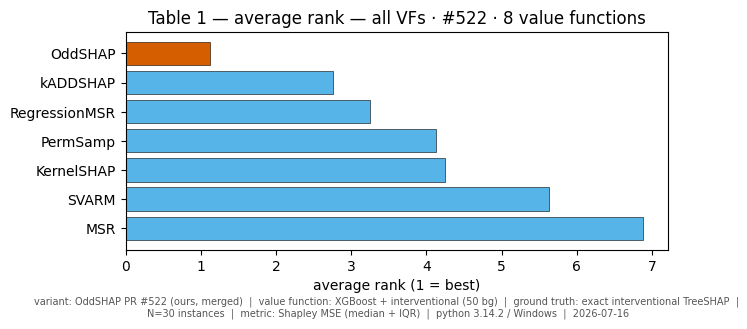
\includegraphics[width=0.86\textwidth]{figures/oddshap-rank-table.png}
    \caption[Average rank across the eight value functions]{%
        \textbf{Average rank} (the paper's Table~1), PR~\#522. Lower is better; rank~1 is the
        lowest median MSE on a value function. \oddshap{} averages 1.125 over the six baselines
        shown --- not comparable with the paper's 1.50, see below.}
    \label{fig:oddshap:rank}
\end{figure}

\begin{figure}[tbp]
    \centering
    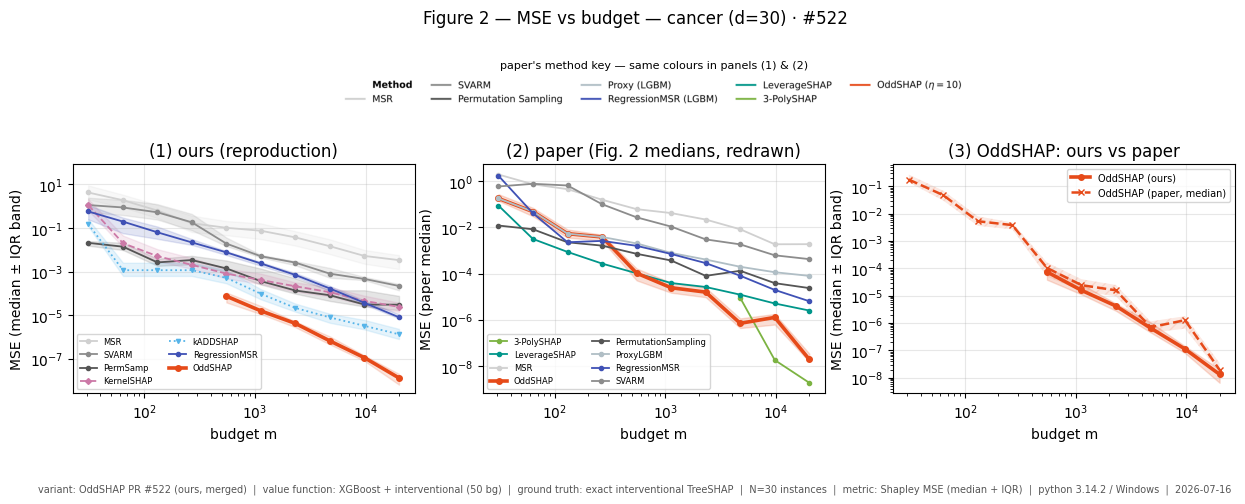
\includegraphics[width=\textwidth]{figures/oddshap-fig2-first.png}
    \caption[MSE against budget, ours against the paper's]{%
        \textbf{MSE against budget on Cancer ($d=30$)}, reproducing the paper's Figure~2.
        Log--log; median over 30 predictions, band is the IQR.
        \textbf{(1)} ours, against \shapiq{}'s six baselines. \textbf{(2)} the paper's medians,
        redrawn --- a different method set, hence not a like-for-like overlay.
        \textbf{(3)} \oddshap{} alone: ours (solid) against the paper's digitised median
        (dashed).}
    \label{fig:oddshap:fig2}
\end{figure}

\begin{figure}[tbp]
    \centering
    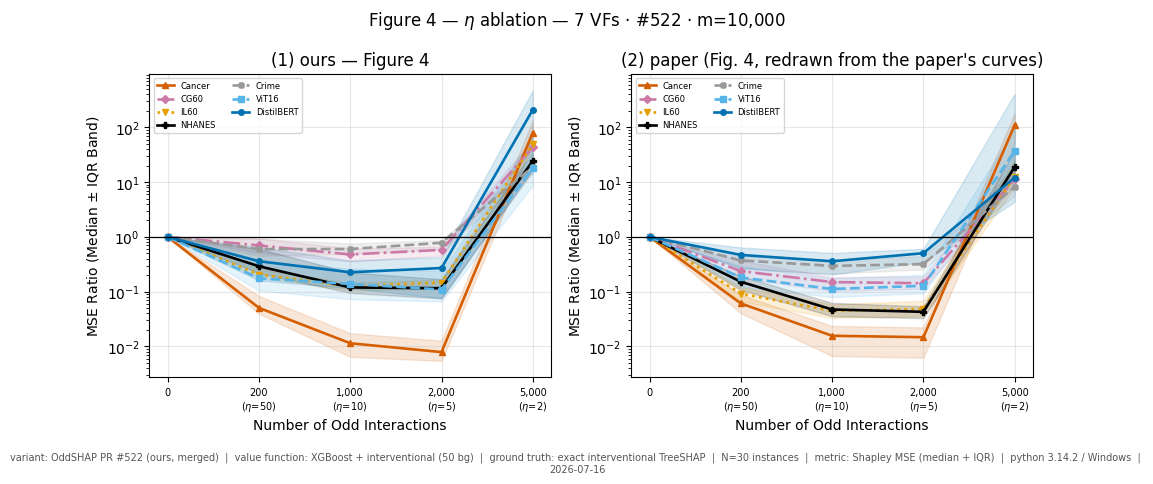
\includegraphics[width=\textwidth]{figures/oddshap-fig4-eta.png}
    \caption[The interaction ablation]{%
        \textbf{The interaction ablation} (the paper's Figure~4) at $m = 10{,}000$, seven value
        functions --- Estate excluded, as the paper excludes it. $y$: MSE \emph{ratio} against
        the interaction-free baseline, so $1.0$ means the interactions changed nothing.
        $x$: odd interactions admitted, fixed by $\lceil m/\eta \rceil$; the annotated $\eta$
        runs from 50 (few) to 2 (many). \textbf{(1)} ours, \textbf{(2)} the paper's, redrawn.}
    \label{fig:oddshap:fig4}
\end{figure}

\paragraph{Reading the average rank.}
Our 1.125 should not be read against the paper's 1.50 as an improvement. The two averages are
taken over different baseline pools: ours over the six baselines in the configuration table,
the paper's over a larger set that also includes \leverageshap{}, \polyshap{}, FourierSHAP and
the fixed-budget FFD variants. A smaller pool makes rank~1 easier to hold. The number
reproduces the \emph{ordering}, not the value.

\paragraph{The two variants.}
PR~\#560 relaxes the minimum budget from $n\eta$ to $\eta$ and merges paired regression rows.
Above the minimum budget the two agree to machine precision --- the largest relative deviation
across the tabular value functions is of order $10^{-12}$, and on the two deep-learning value
functions they agree bitwise. Every paper-scale result is therefore unchanged by the follow-up;
its entire effect is confined to the low-budget regime in which PR~\#522 refuses.

\paragraph{Honest gaps.}
The two deep-learning value functions are budget-truncated: ViT-16 reaches a budget of 1{,}895
and DistilBERT 1{,}591, rather than the paper's sweep to $\min(2^d, 20\,000)$. Both are
low-dimensional ($d = 16$, $d = 14$) --- the regime in which the paper itself reports
convergence between the methods --- and the $\eta$ ablation is complete for both. The
high-budget tail for these two is nevertheless not confirmed here. Separately, the reference
curves in
\texttt{paper\_reference/} are digitised from the published figures rather than taken from
author-provided numbers, and are accurate only to the resolution of that source.
